\documentclass[border=10pt]{standalone}

\usepackage{tikz}
\usepackage{tikzsymbols}
\usetikzlibrary{calc,patterns,shapes.geometric}

\def\centerarc[#1](#2)(#3:#4:#5){\draw[#1] ($(#2)+({#5*cos(#3)},{#5*sin(#3)})$) arc (#3:#4:#5);}

\begin{document}
	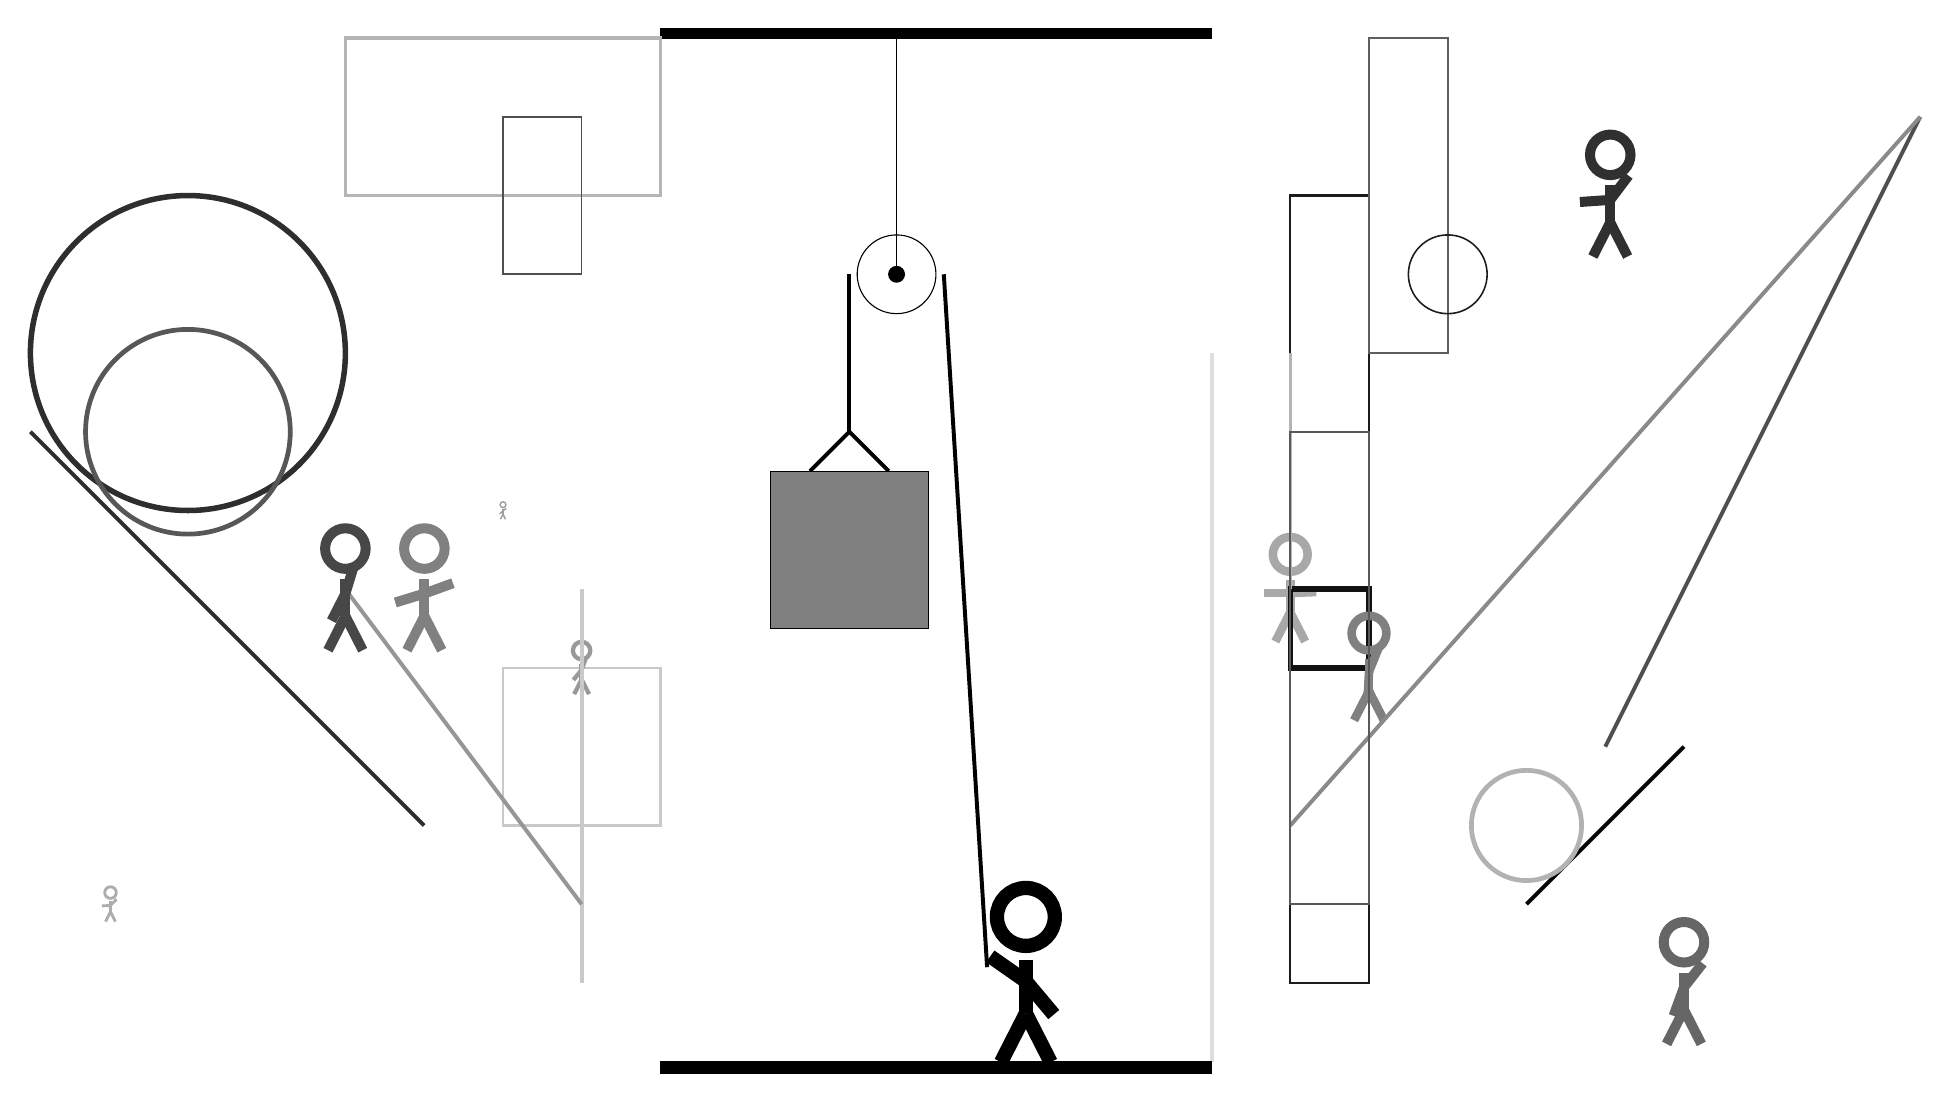
\begin{tikzpicture}
		%%%%% START %%%%%
		
		\draw[fill=black] (-2, 10) rectangle (5, 10.125);
		
		\draw (1, 7) circle (0.5);
		\draw[fill=black] (1, 7) circle (0.1);
		\draw (1, 10) -- (1, 7);
		
		\draw[line width=0.5mm] (-0.1, 4.5) -- (0.4, 5.0) -- (0.9, 4.5);
		\draw[fill=black!50] (-0.6, 4.5) rectangle (1.4, 2.5);
		
		\node[line width=0.6mm, color=black!34] at (6, 3) {\Strichmaxerl[6][0][2]};
		
		\draw[line width=0.7mm, color=black!93] (7, 3) rectangle (6, 2);
		\draw[line width=0.3mm, color=black!21] (-2, 2) rectangle (-4, 0);
		\node[line width=0.7mm, color=black!50] at (-5, 3) {\Strichmaxerl[7][17][20]};
		\node[line width=0.5mm, color=black!50] at (7, 2) {\Strichmaxerl[6][87][68]};
		\draw[line width=0.5mm, color=black!82](-5, 0) -- (-10, 5);
		\draw[line width=0.5mm, color=black!98](9, -1) -- (11, 1);
		
		\node[line width=0.6mm, color=black!40] at (-3, 2) {\Strichmaxerl[3][51][70]};
		\draw[line width=0.3mm, color=black!89] (6, -2) rectangle (7, 8);
		\node[line width=0.3mm, color=black!38] at (-4, 4) {\Strichmaxerl[1][38][43]};
		\draw[line width=0.5mm, color=black!69](10, 1) -- (14, 9);
		\draw[line width=0.3mm, color=black!63] (7, 10) rectangle (8, 6);
		\node[line width=0.6mm, color=black!60] at (11, -2) {\Strichmaxerl[7][70][52]};
		\draw[line width=0.5mm, color=black!21] (-3, 3) rectangle (-3, -2);
		\draw[line width=0.5mm, color=black!13](5, -3) -- (5, 6);
		\draw[line width=0.4mm, color=black!29] (6, 3) rectangle (6, 6);
		
		\draw[line width=0.4mm, color=black!29] (-2, 10) rectangle (-6, 8);
		
		\draw[line width=0.5mm, color=black!41](-3, -1) -- (-6, 3);
		\draw [line width=0.7mm, color=black!82](-8, 6) circle (2.0);
		
		\node[line width=0.3mm, color=black!32] at (-9, -1) {\Strichmaxerl[2][3][46]};
		\draw[line width=0.5mm, color=black!46](6, 0) -- (14, 9);
		
		\draw[line width=0.3mm, color=black!65] (7, 5) rectangle (6, -1);
		\draw [line width=0.6mm, color=black!66](-8, 5) circle (1.3);
		\node[line width=0.3mm, color=black!72] at (-6, 3) {\Strichmaxerl[7][63][73]};
		\draw [line width=0.2mm, color=black!89](8, 7) circle (0.5);
		\node[line width=0.5mm, color=black!81] at (10, 8) {\Strichmaxerl[7][4][53]};
		\draw [line width=0.6mm, color=black!30](9, 0) circle (0.7);
		\draw[line width=0.2mm, color=black!69] (-3, 9) rectangle (-4, 7);
		
		
		\draw[line width=0.5mm] (0.4, 7) -- (0.4, 5.0);
		\centerarc[line width=0.5mm](1, 7)(0:180:0.6);
		\draw[line width=0.5mm](1.6, 7) -- (2.15, -1.8);
		
		\node at (2.6, -1.9) {\Strichmaxerl[10][-35][-50]};
		
		\draw[fill=black] (-2, -3) rectangle (5, -3.15);
		
		%%%%% END %%%%%
	\end{tikzpicture}
\end{document}